\documentclass[12pt]{article}

\title{Symbolic Logic HW 7}
\author{Tyler Tracy}

\usepackage{amsmath}
\usepackage{amssymb}
\usepackage{graphicx}
\graphicspath{ {./imgs/} }

\begin{document}

\maketitle

\section*{Problem 1}

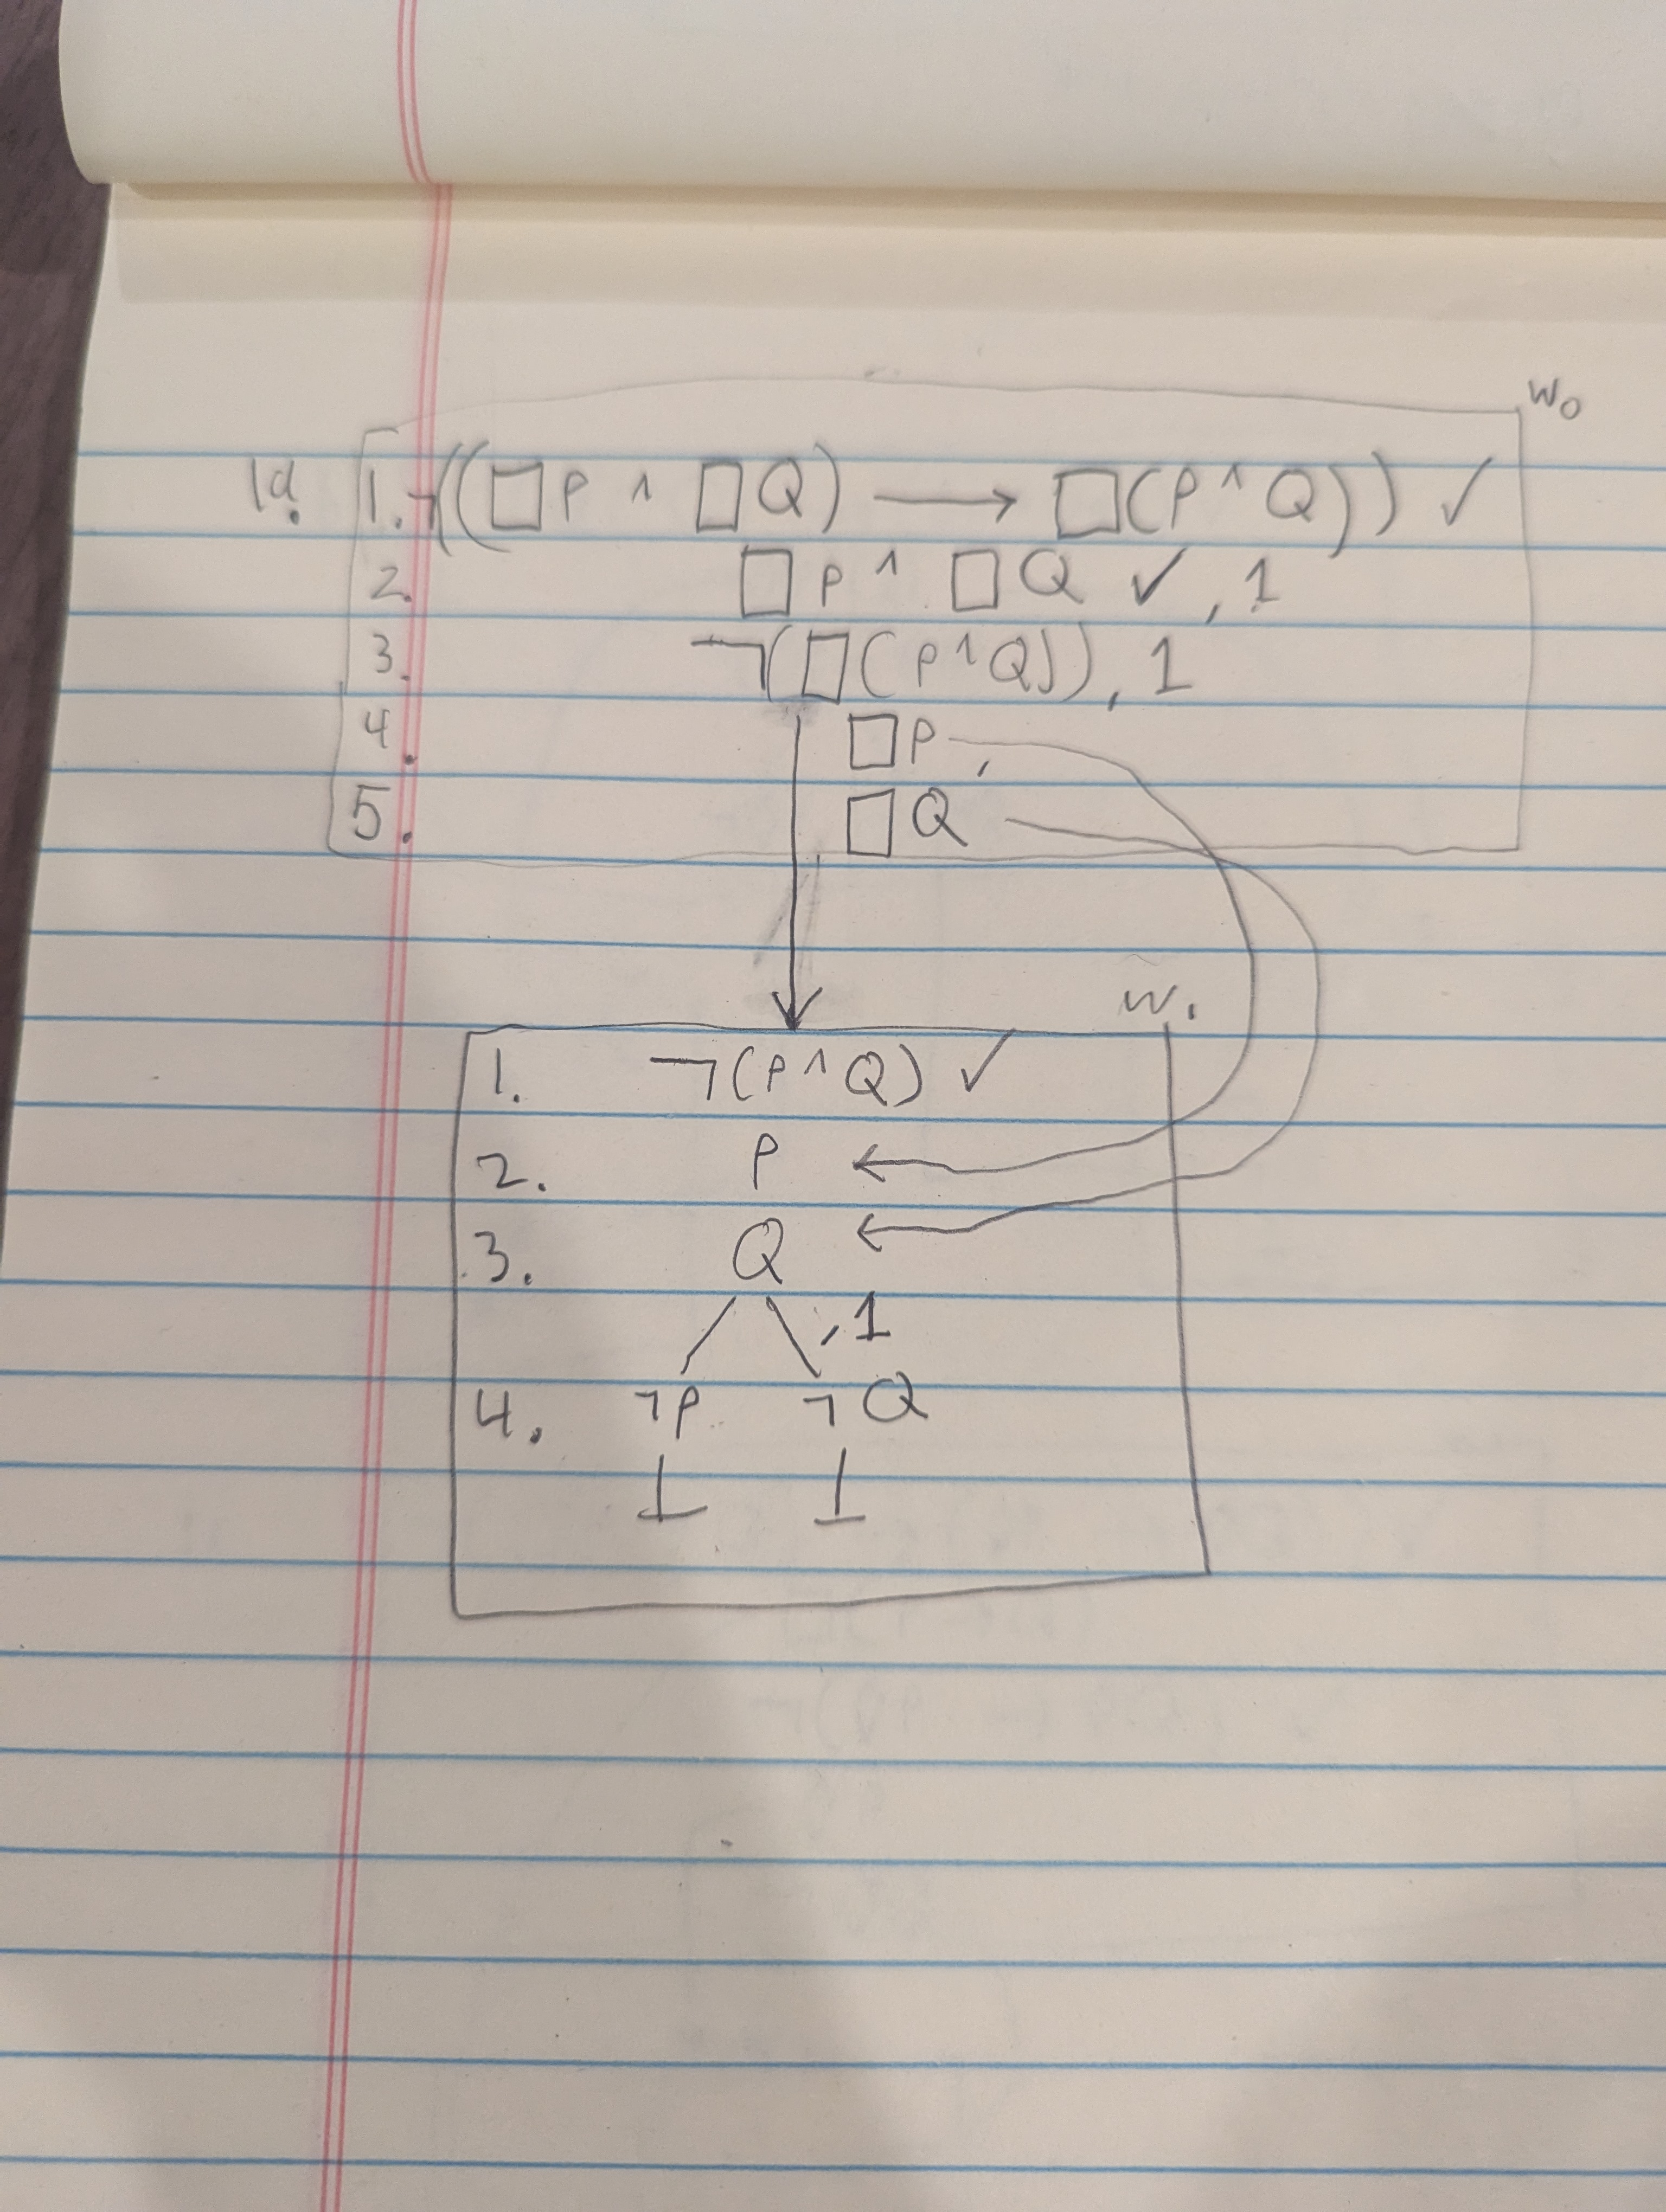
\includegraphics[width=\textwidth]{1a}

\break

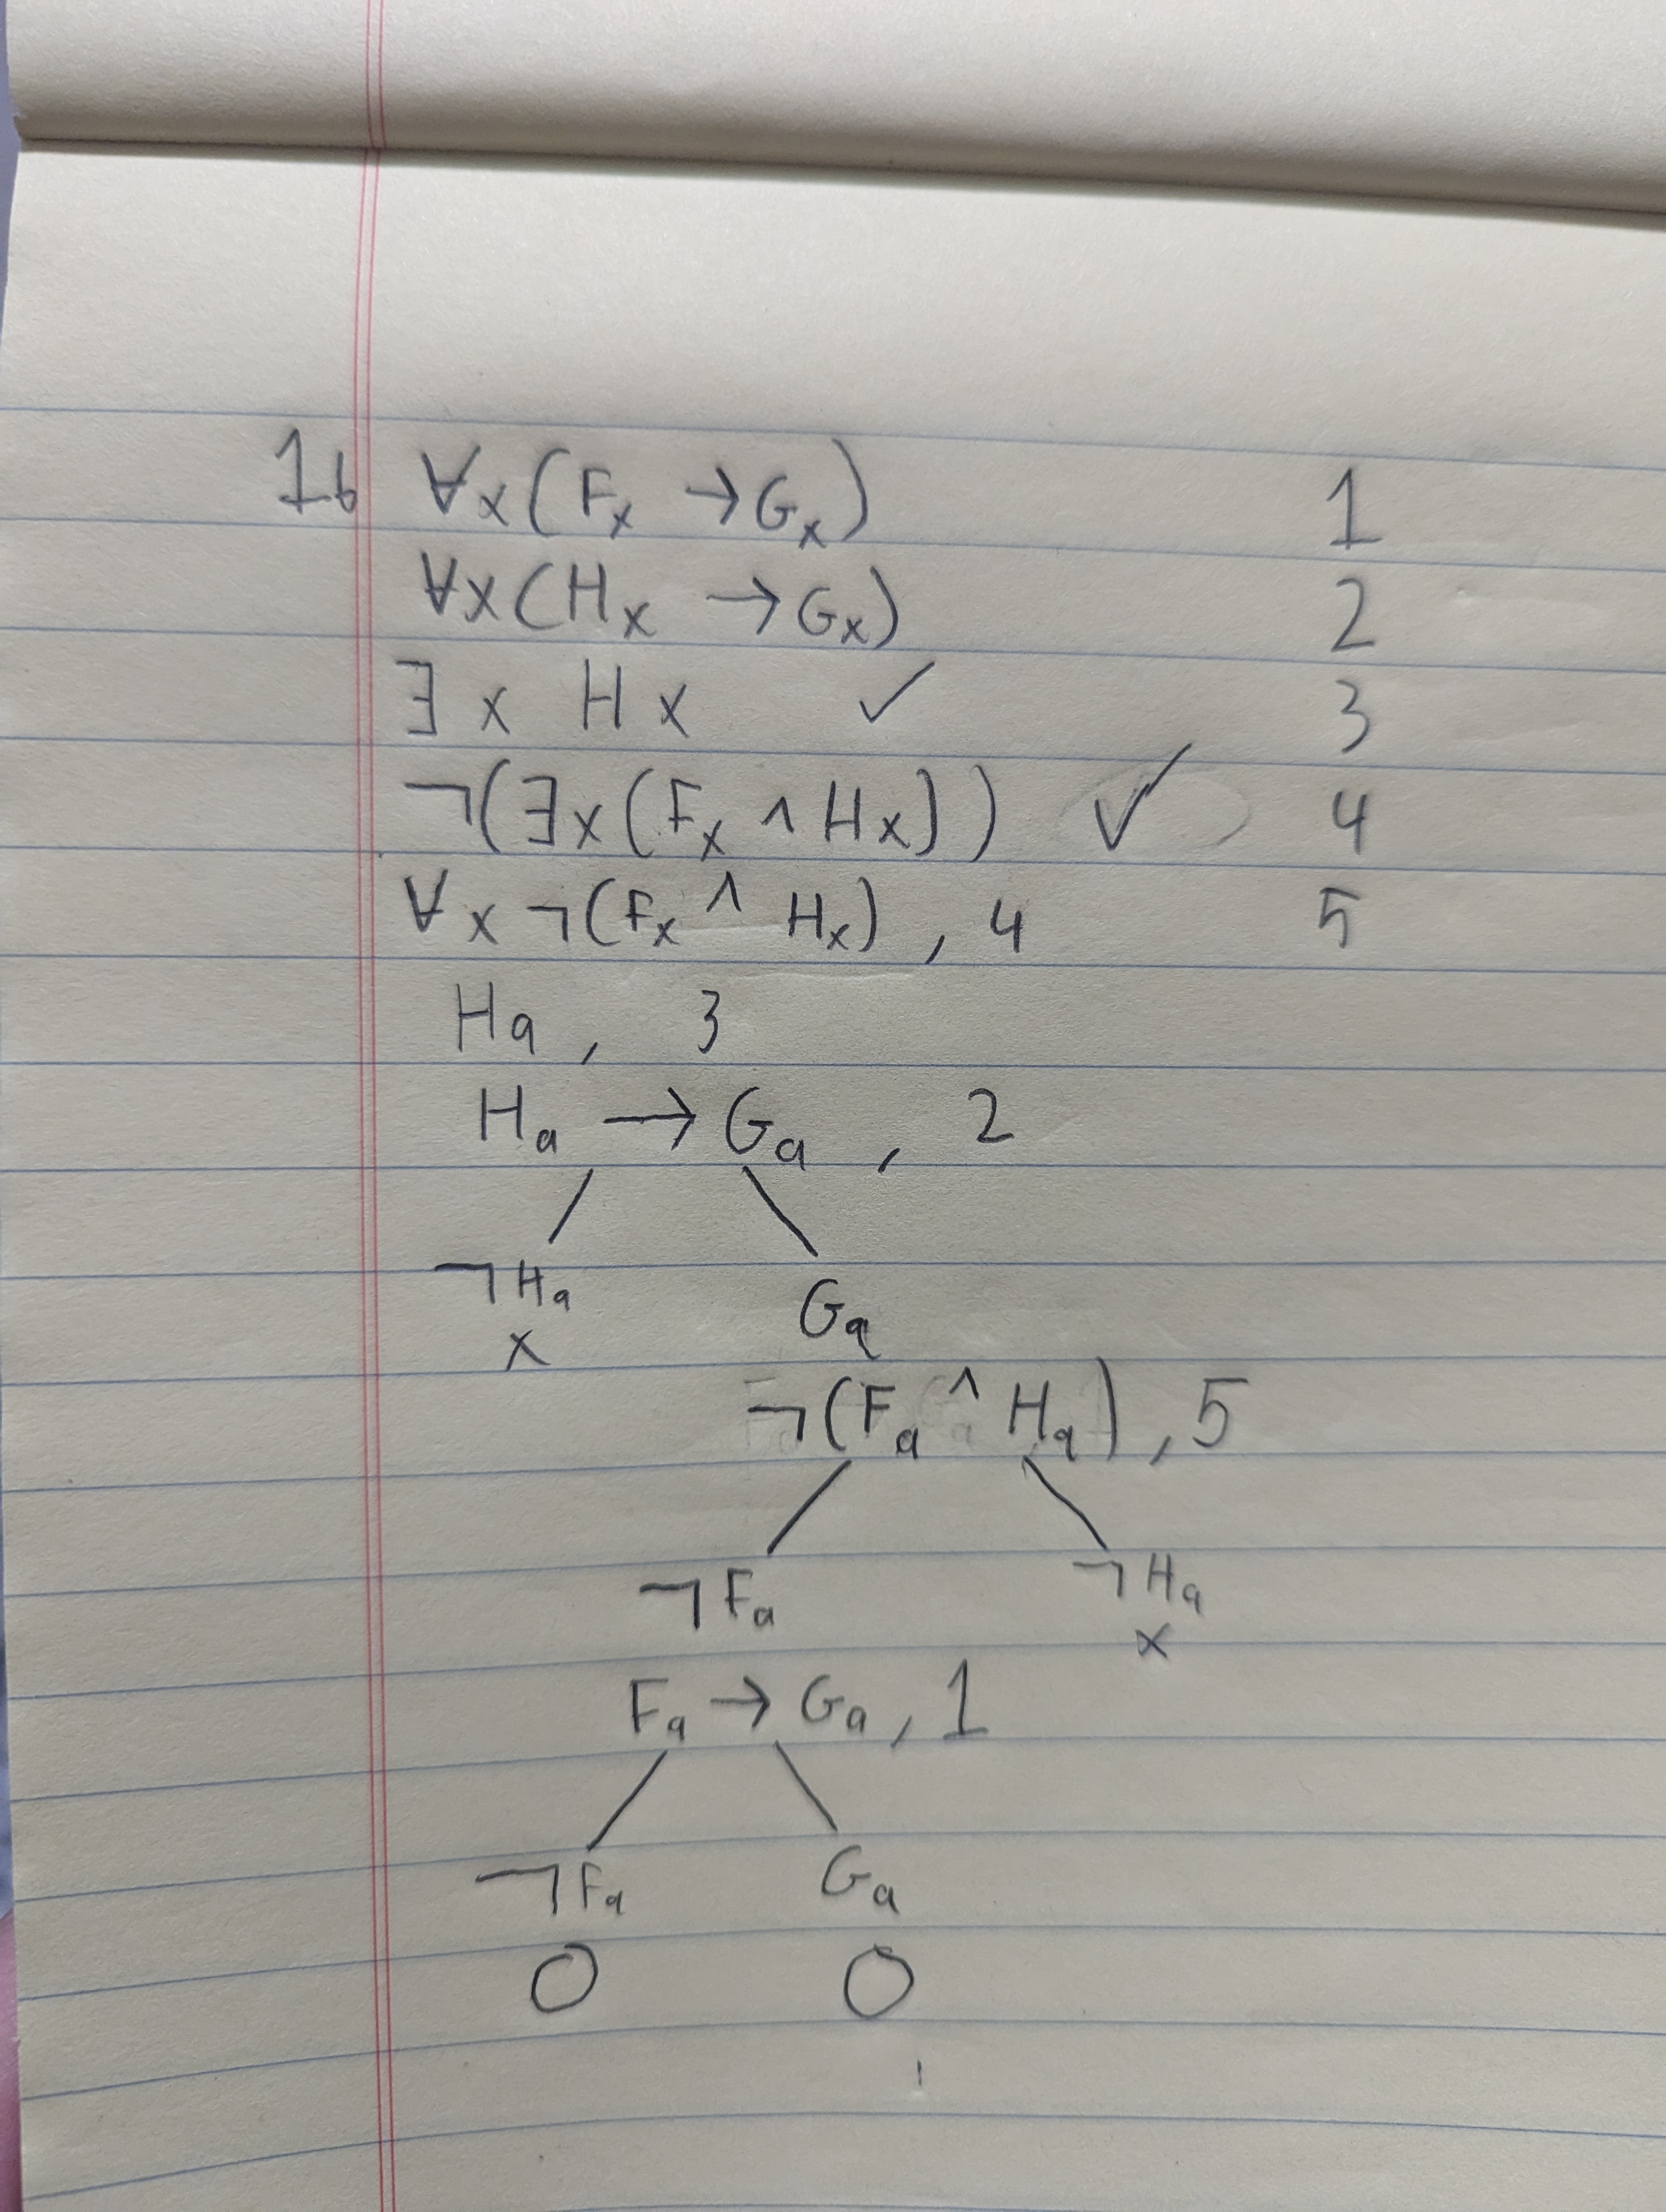
\includegraphics[width=\textwidth]{1b}

\section*{Problem 2}

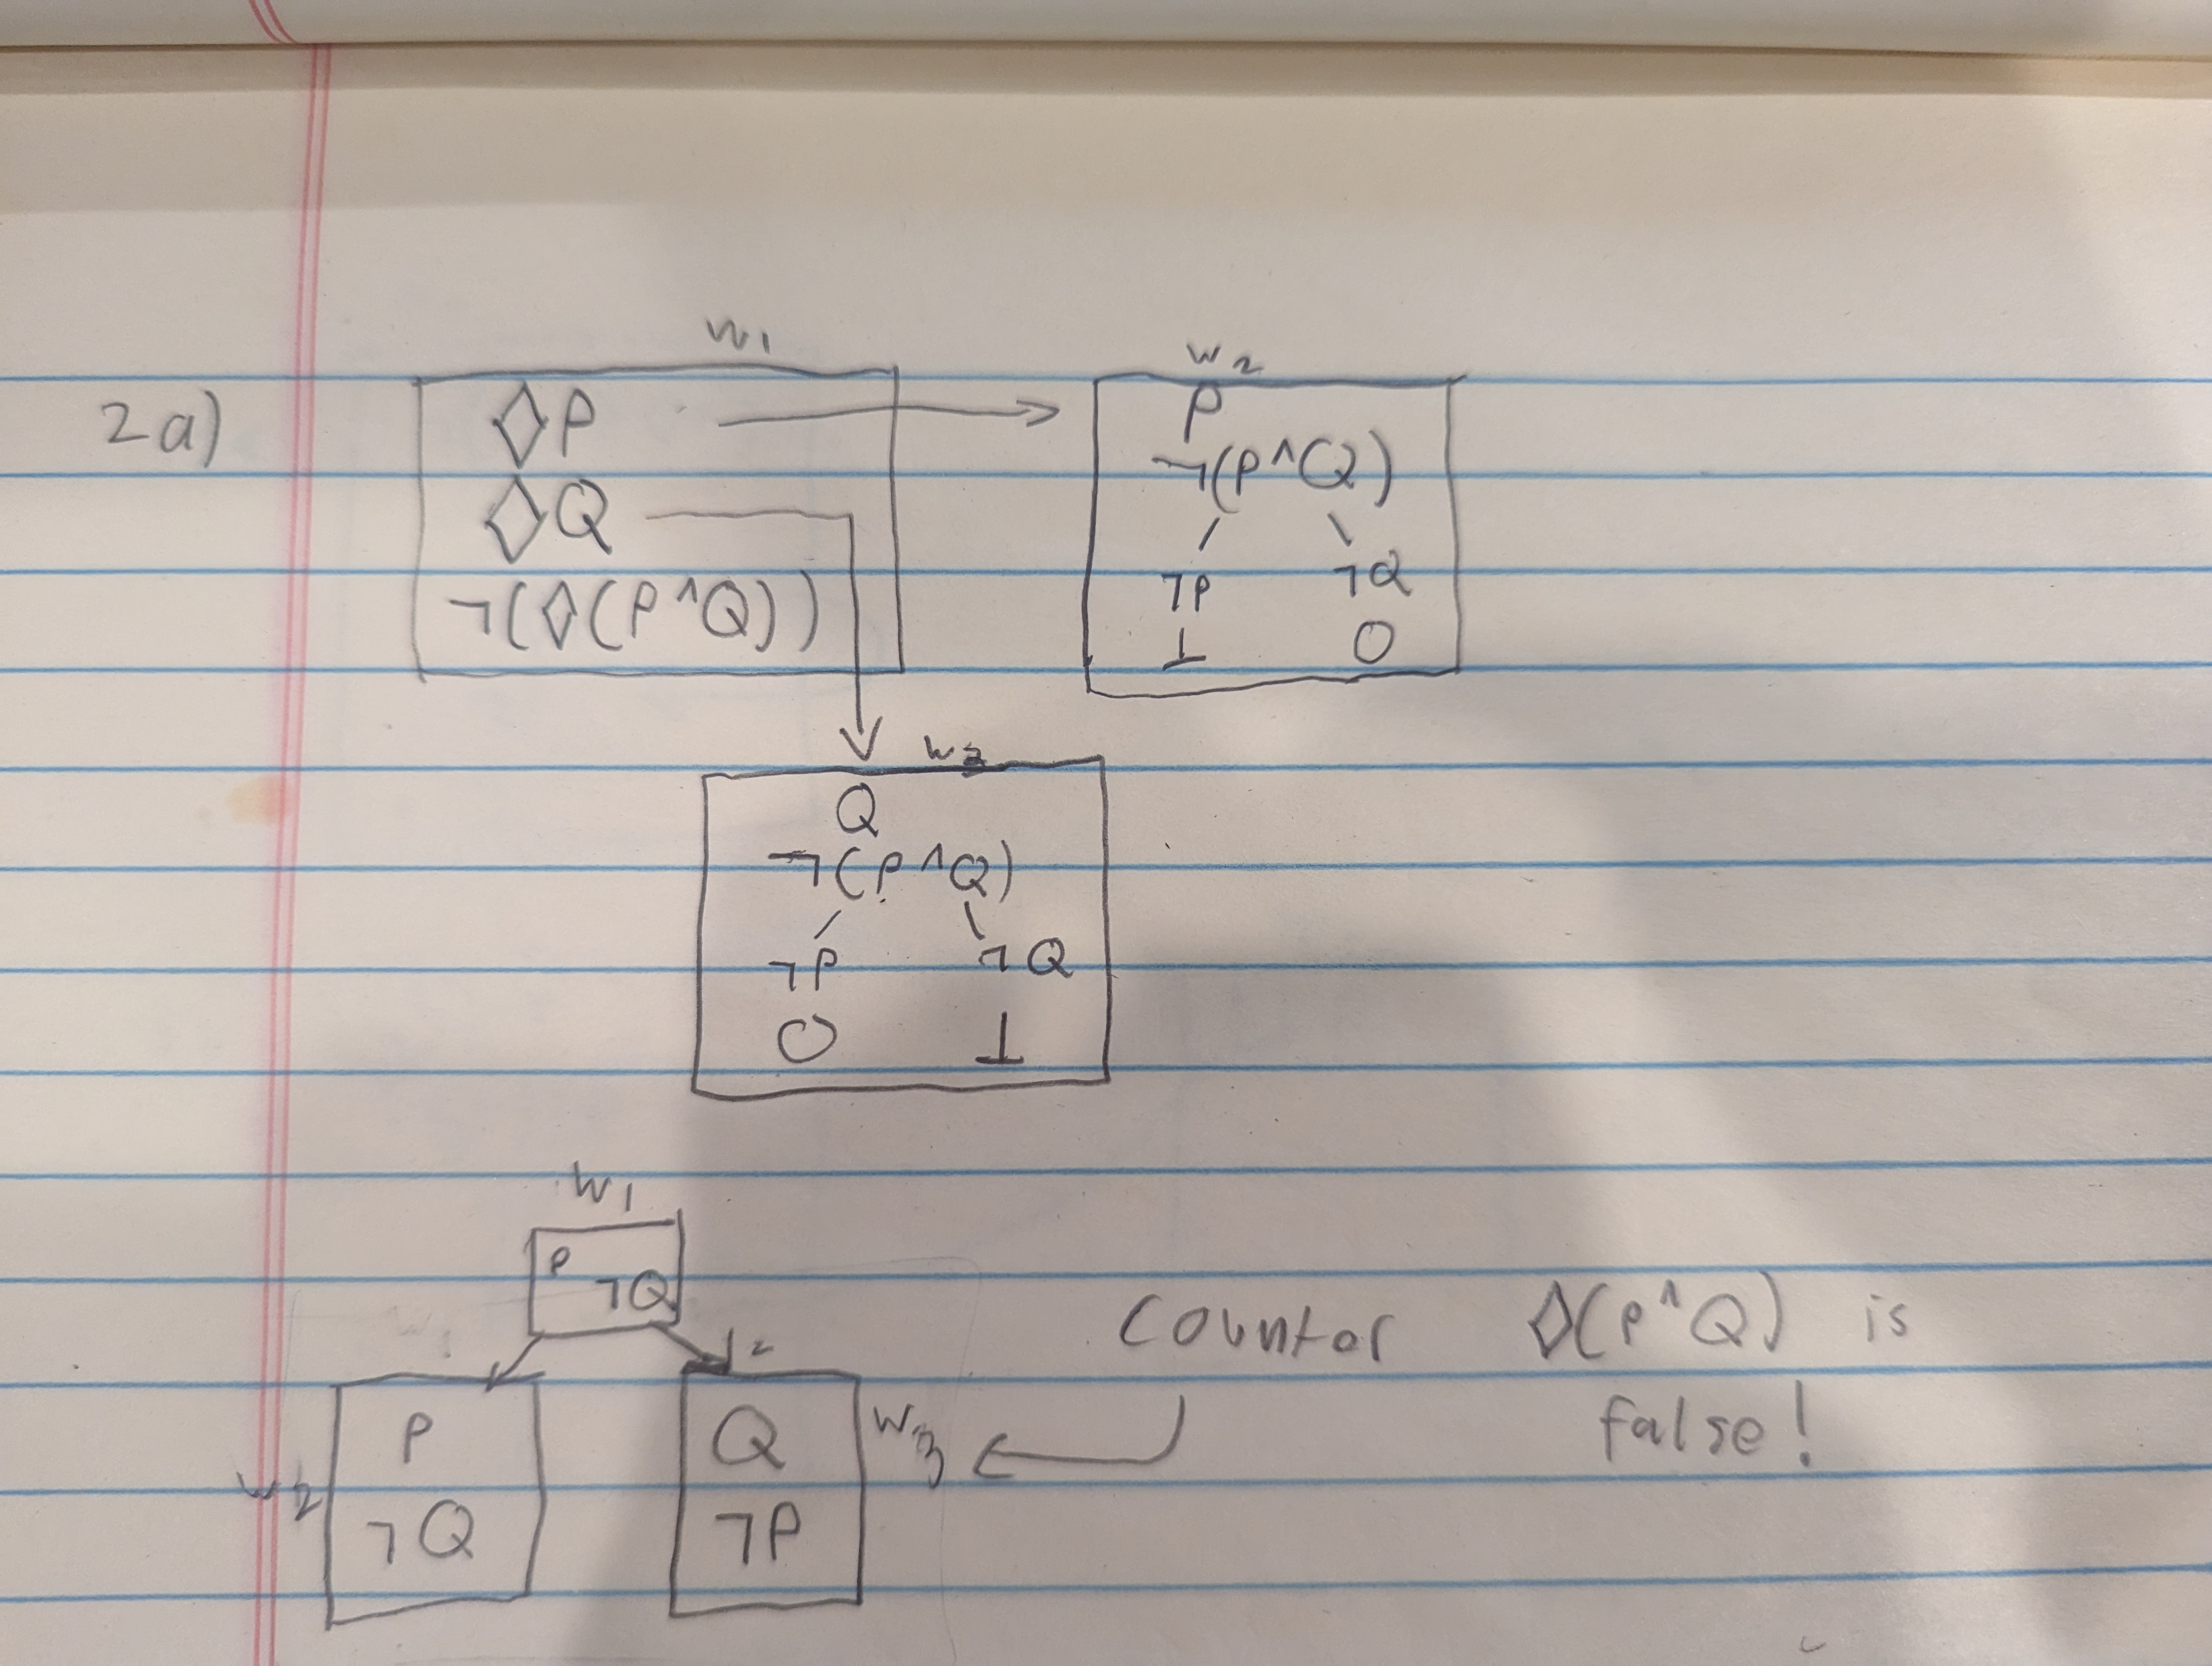
\includegraphics[width=\textwidth]{2a}

\break

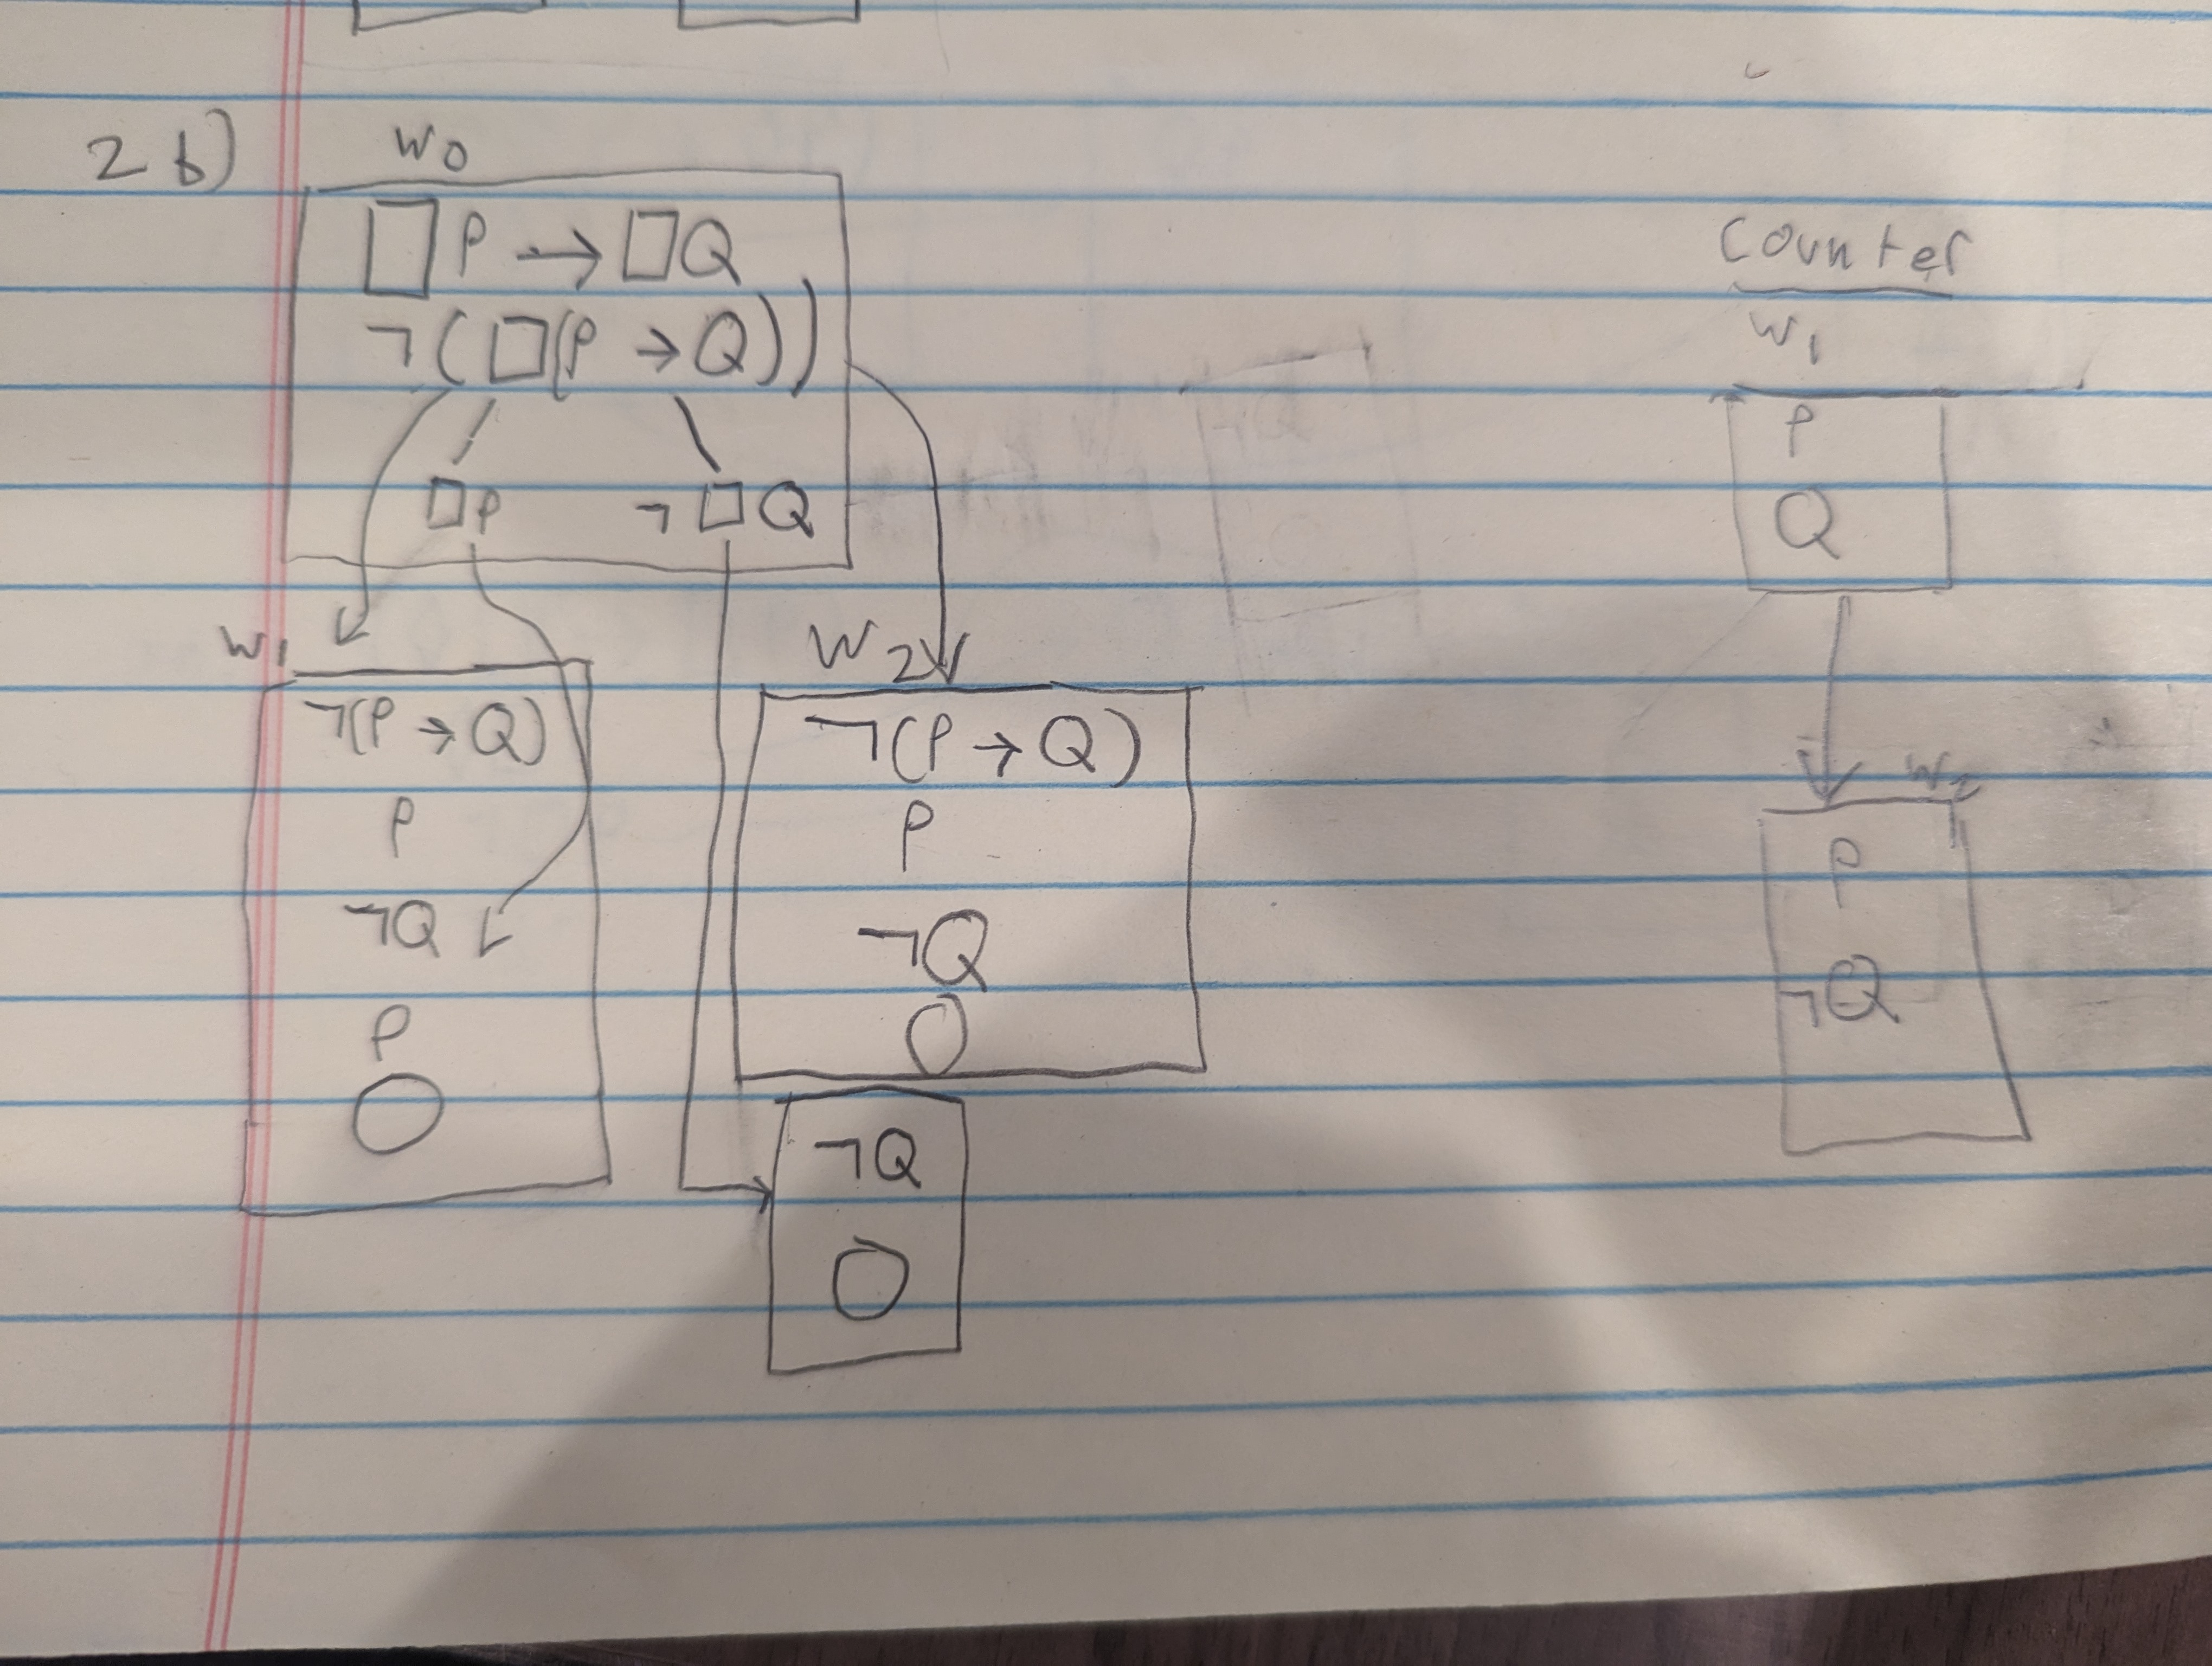
\includegraphics[width=\textwidth]{2b}

\section*{Problem 3}

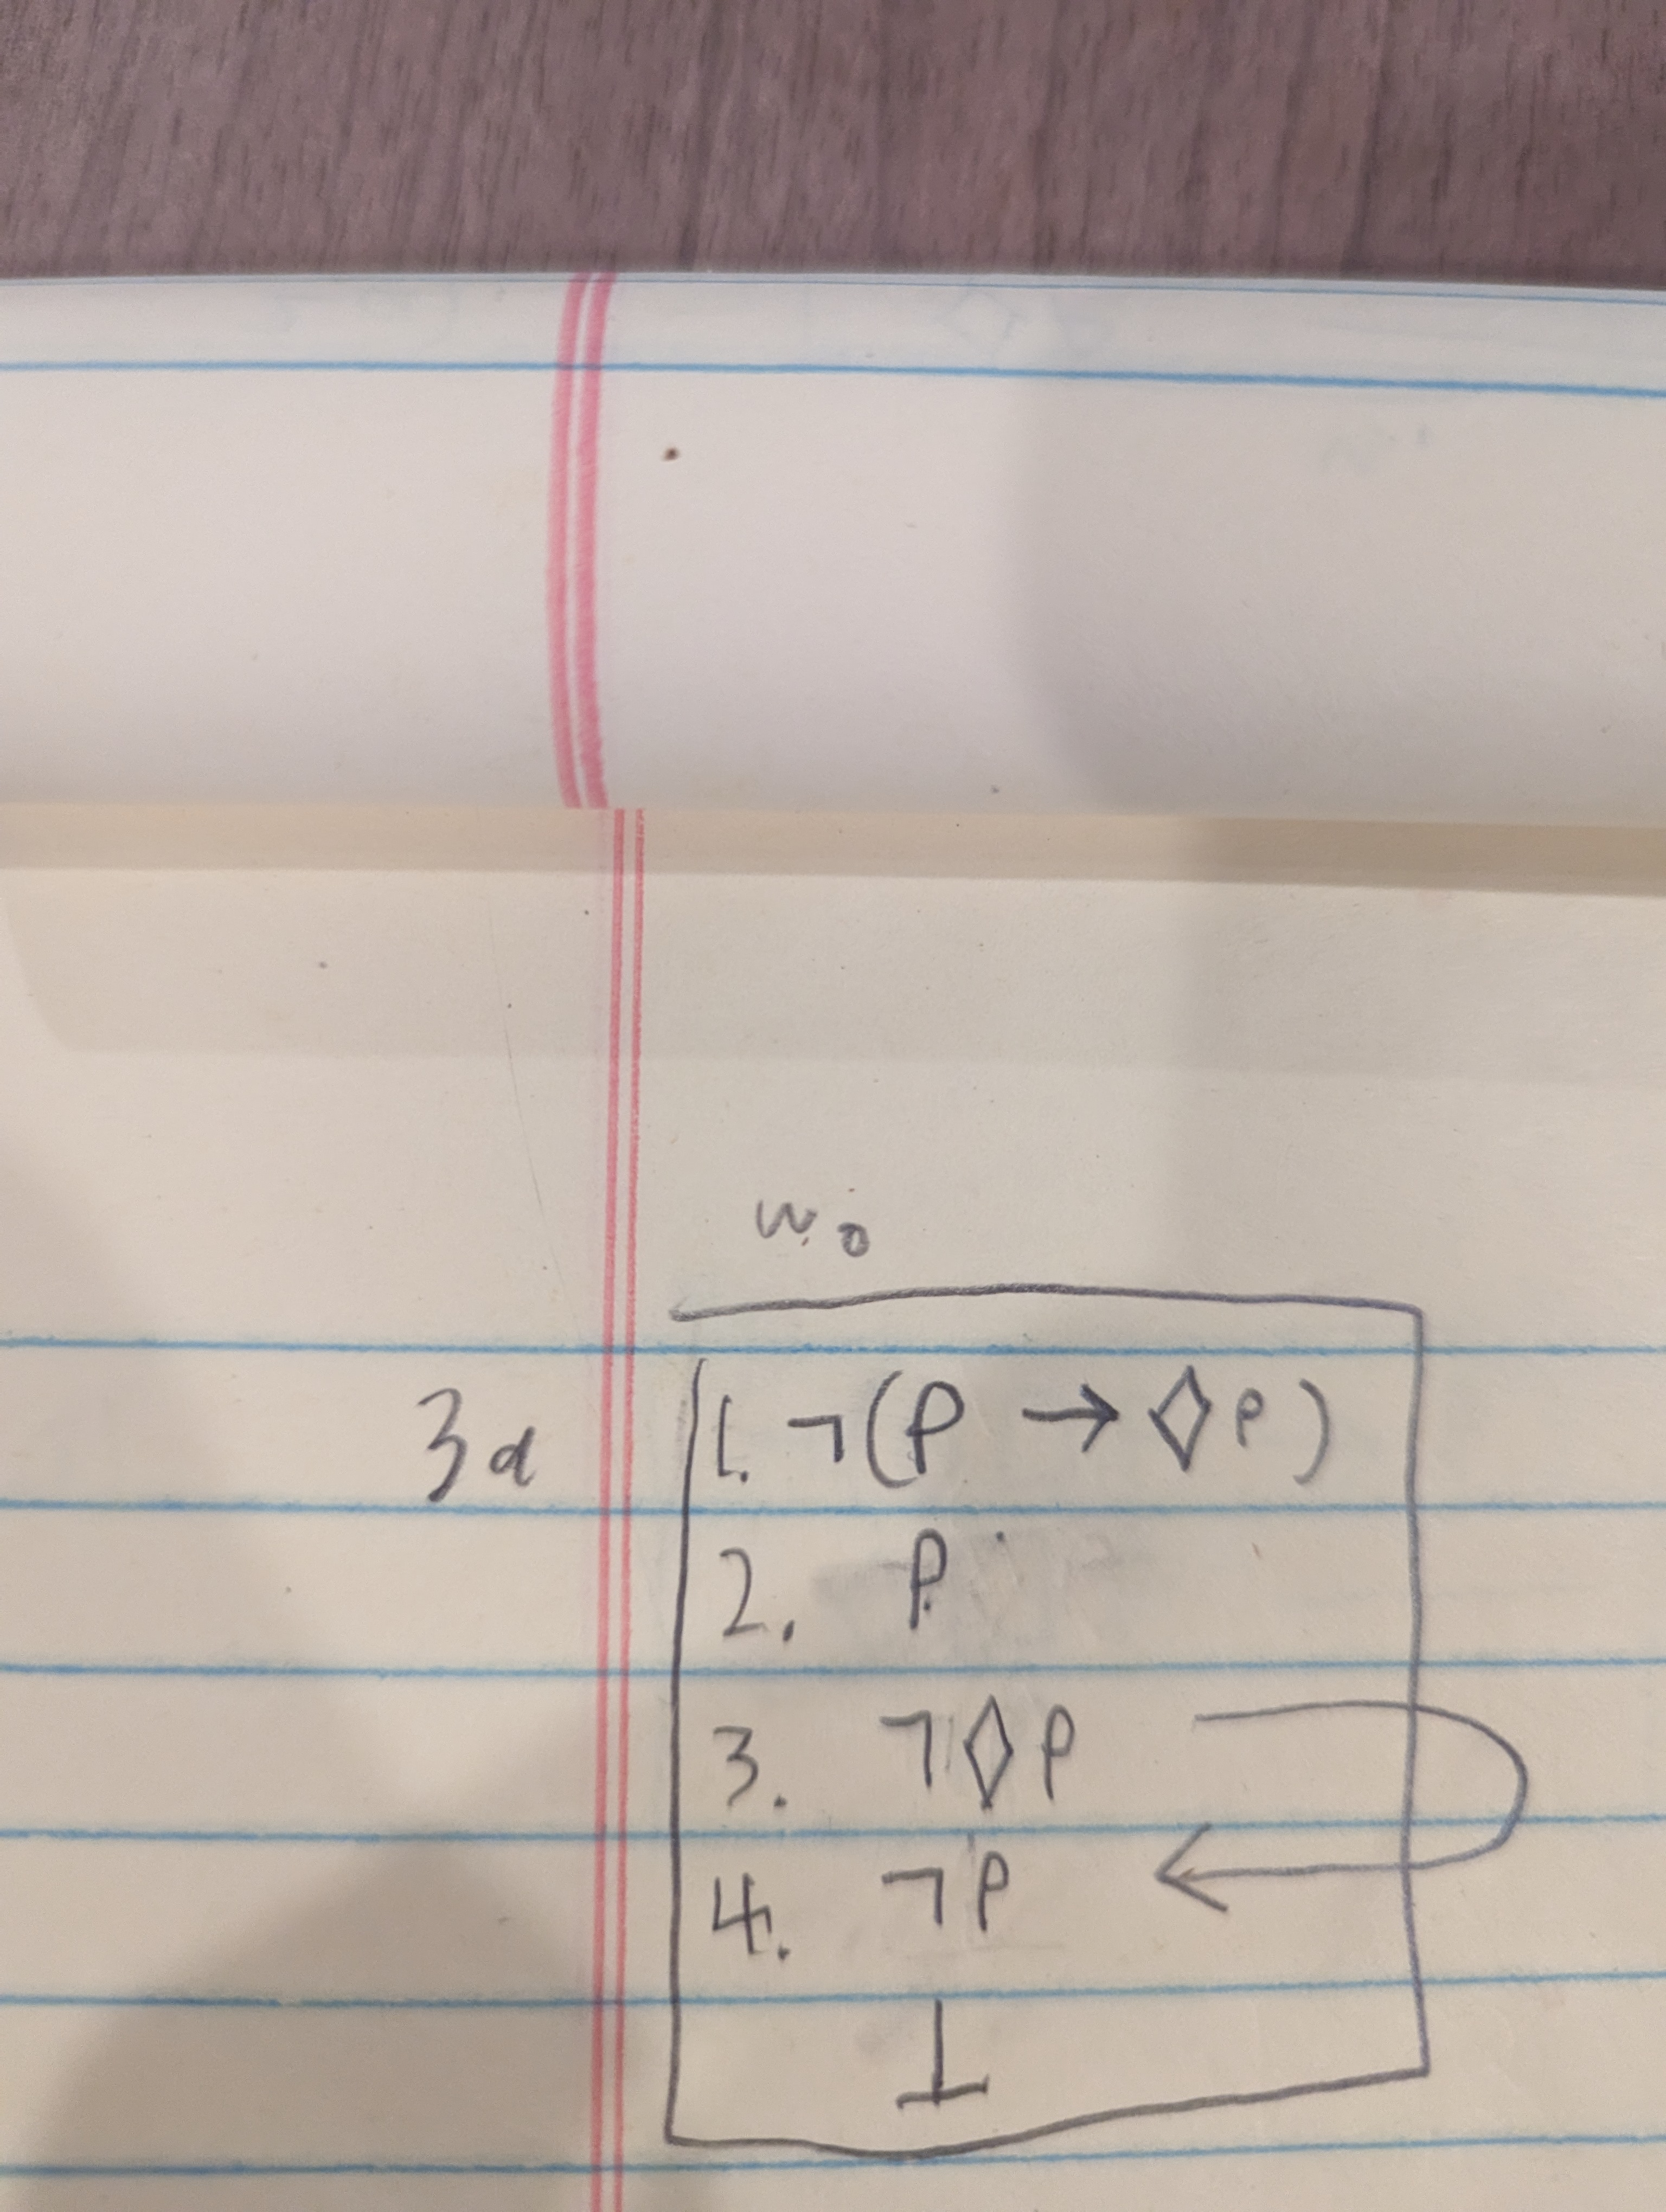
\includegraphics[width=\textwidth]{3a}
\break
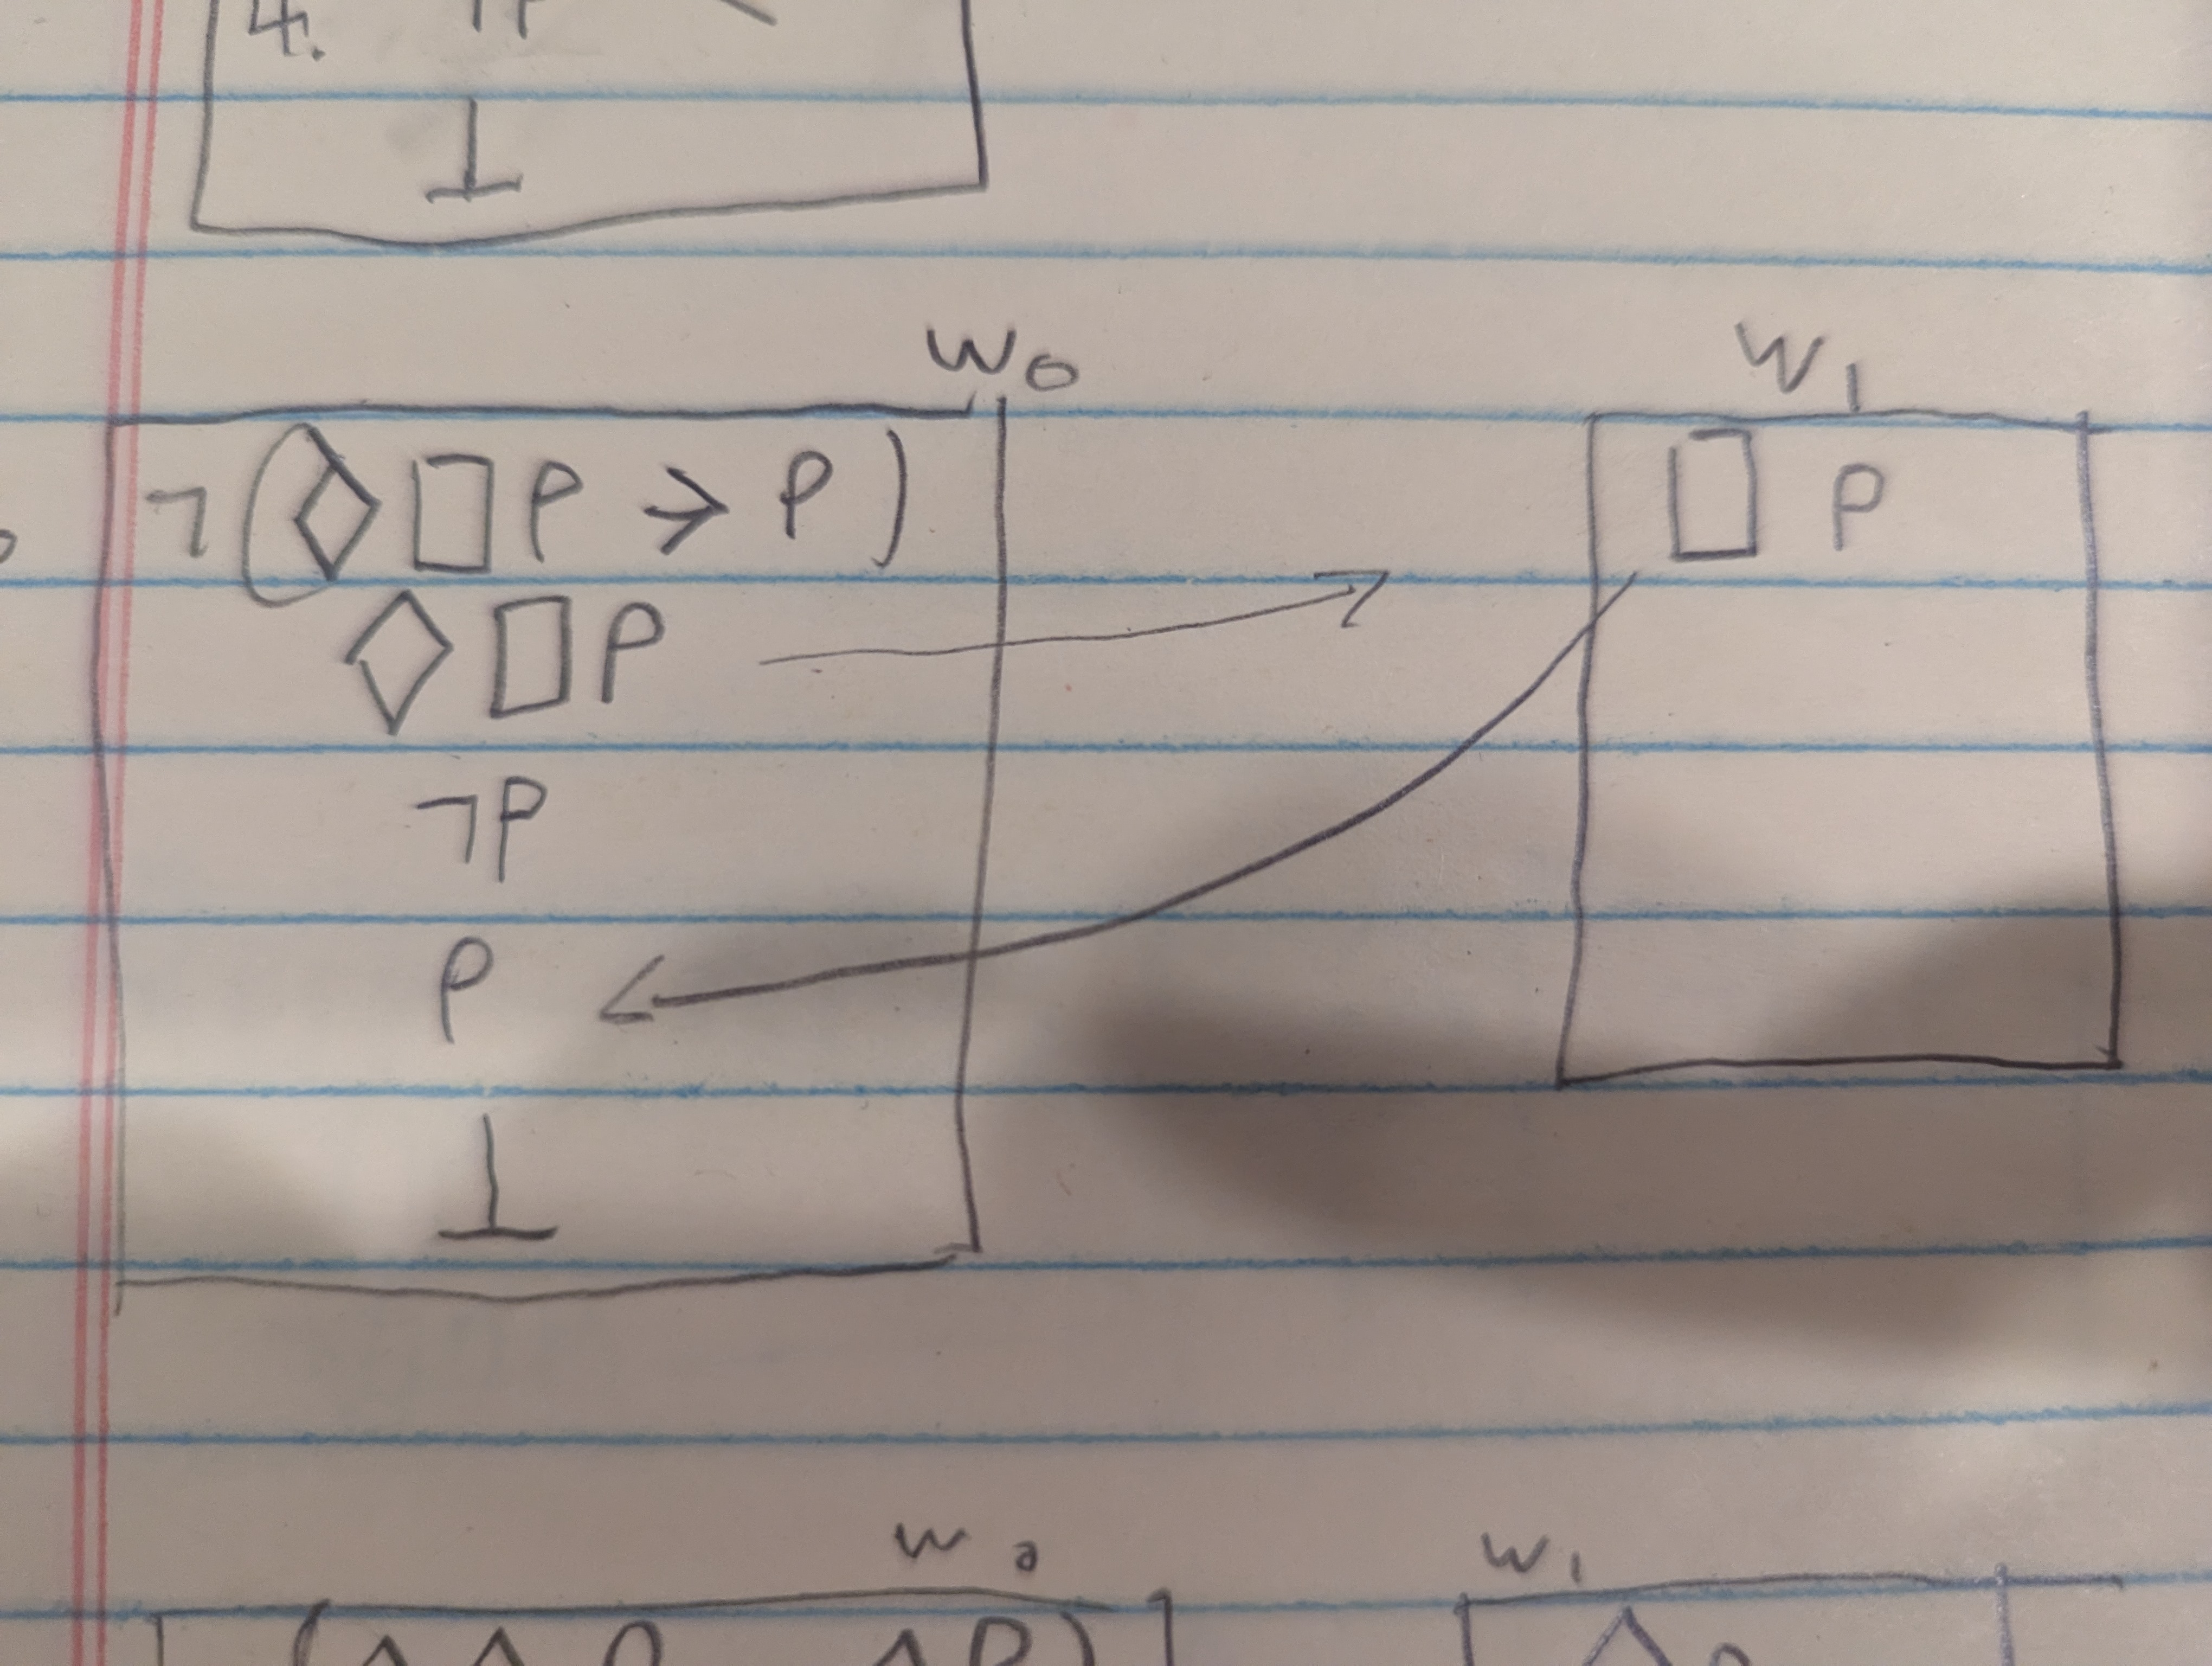
\includegraphics[width=\textwidth]{3b}
\break
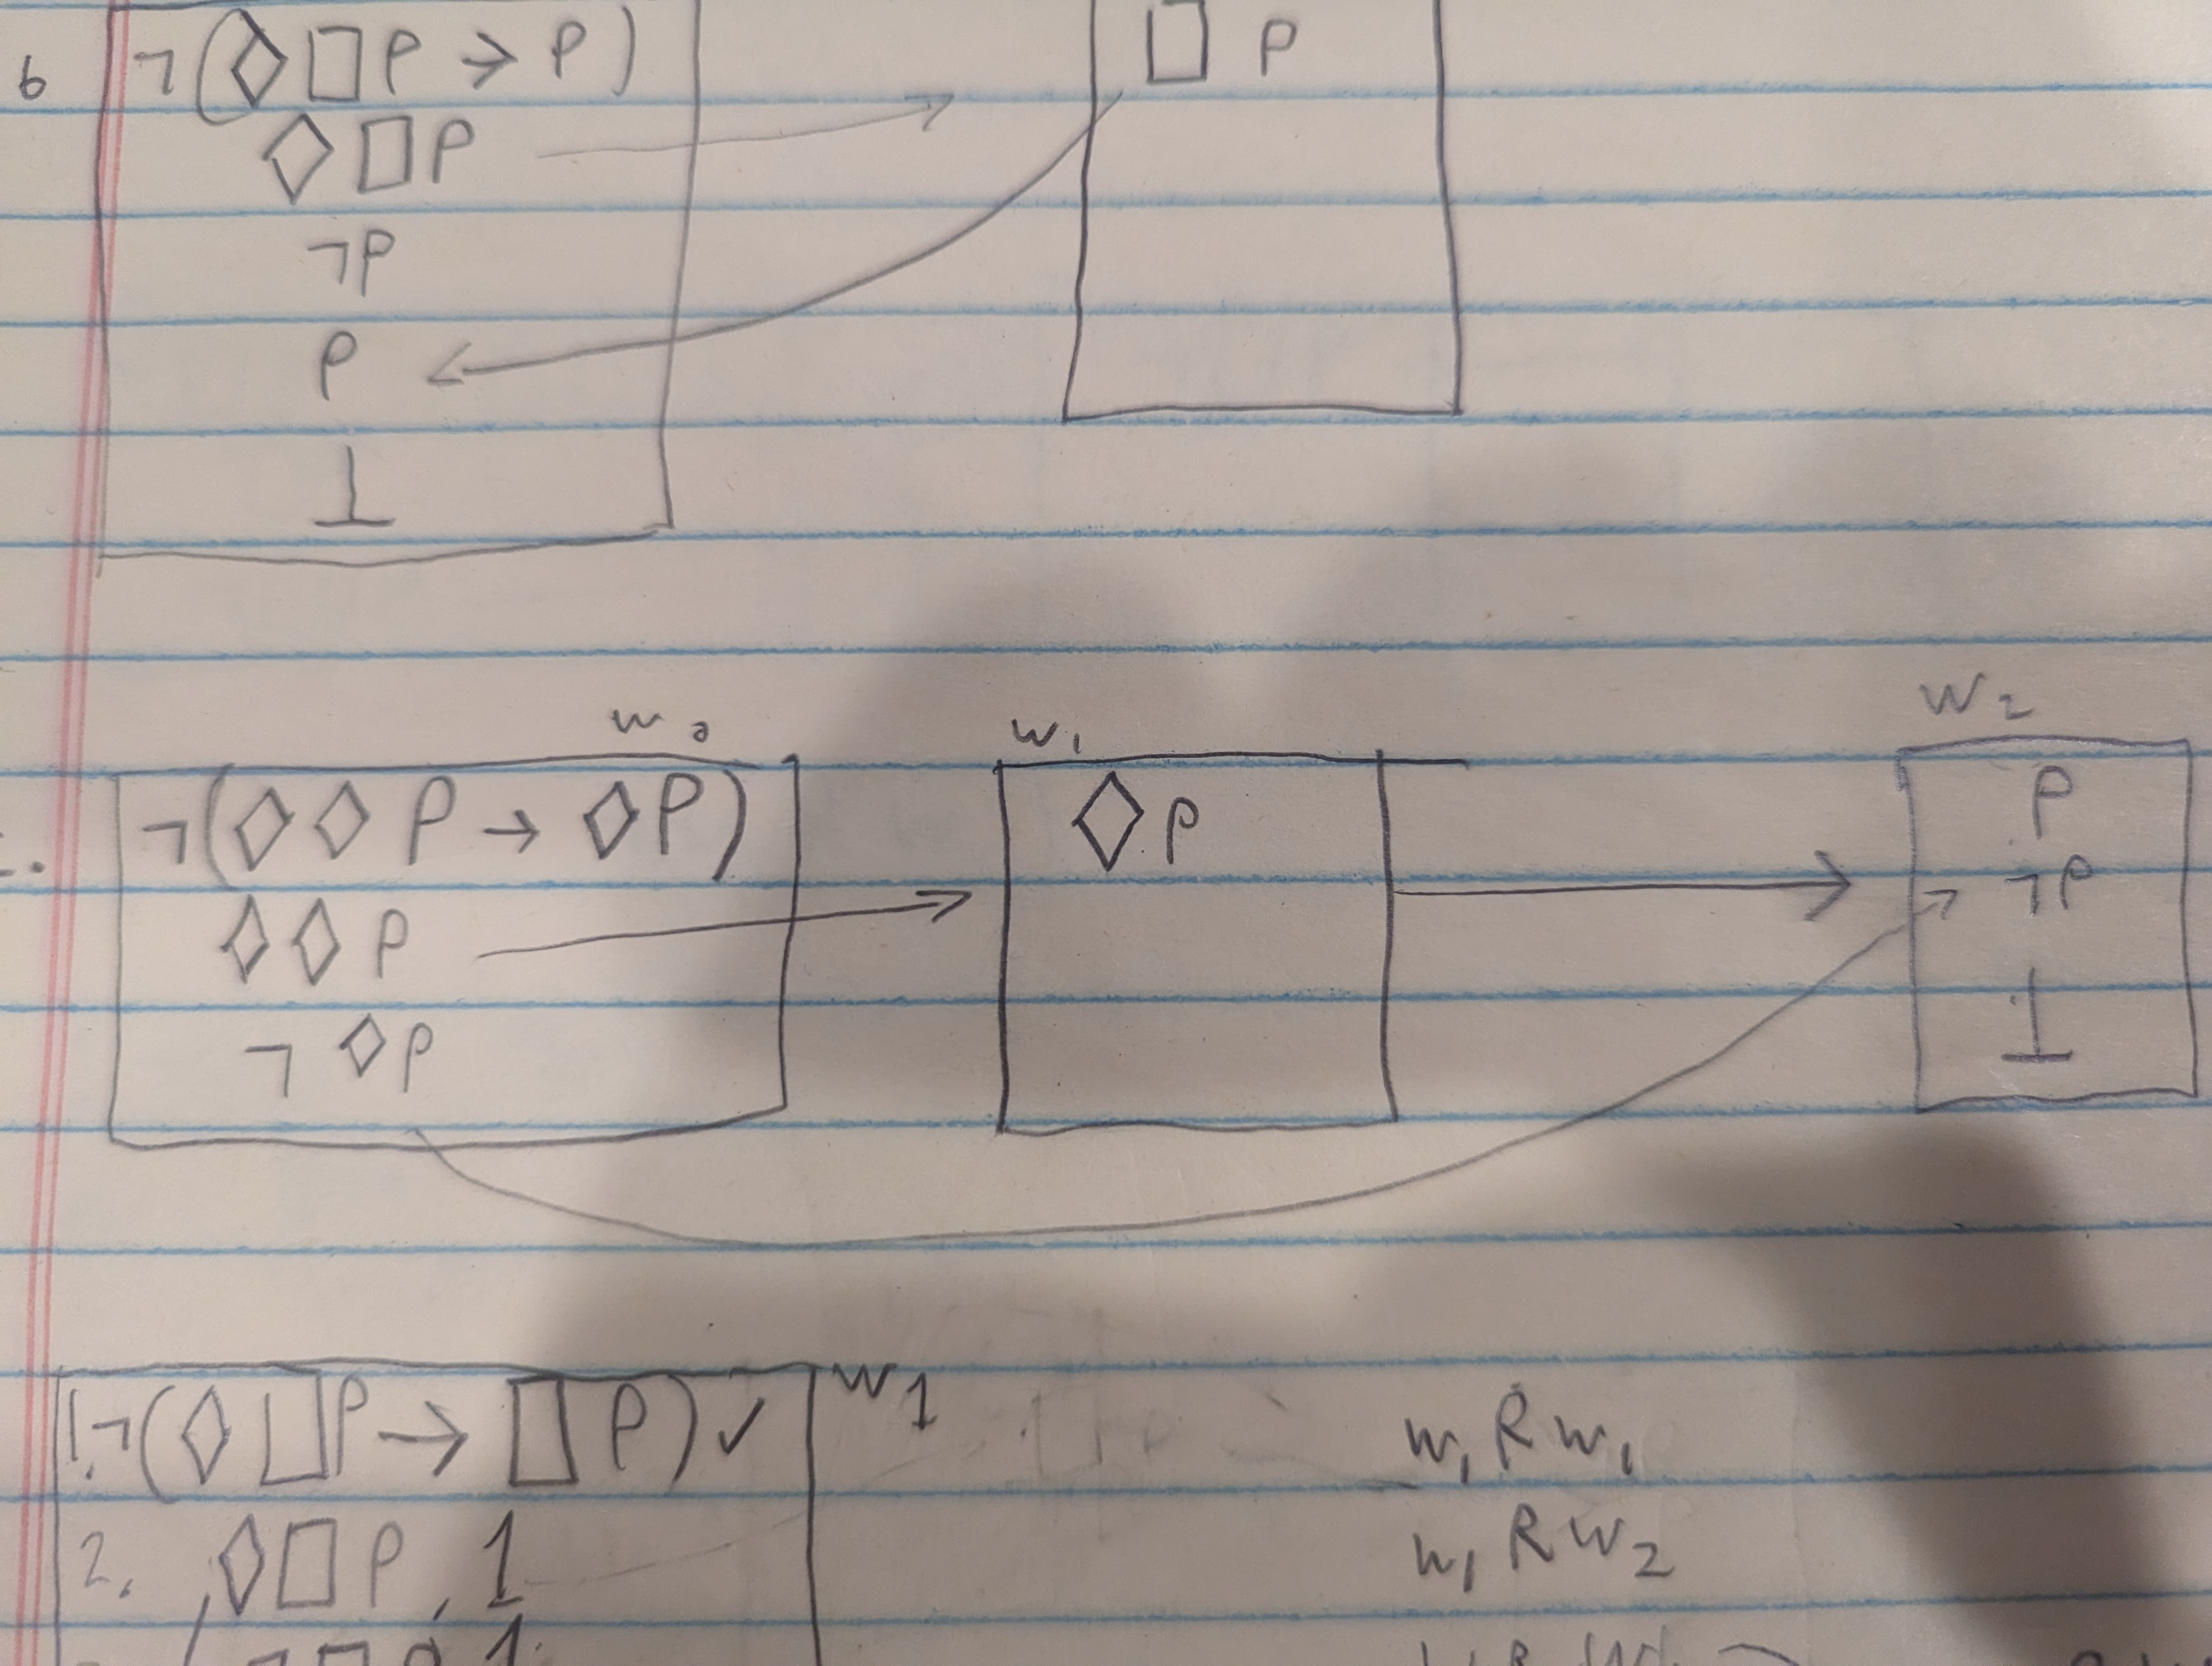
\includegraphics[width=\textwidth]{3c}
\break
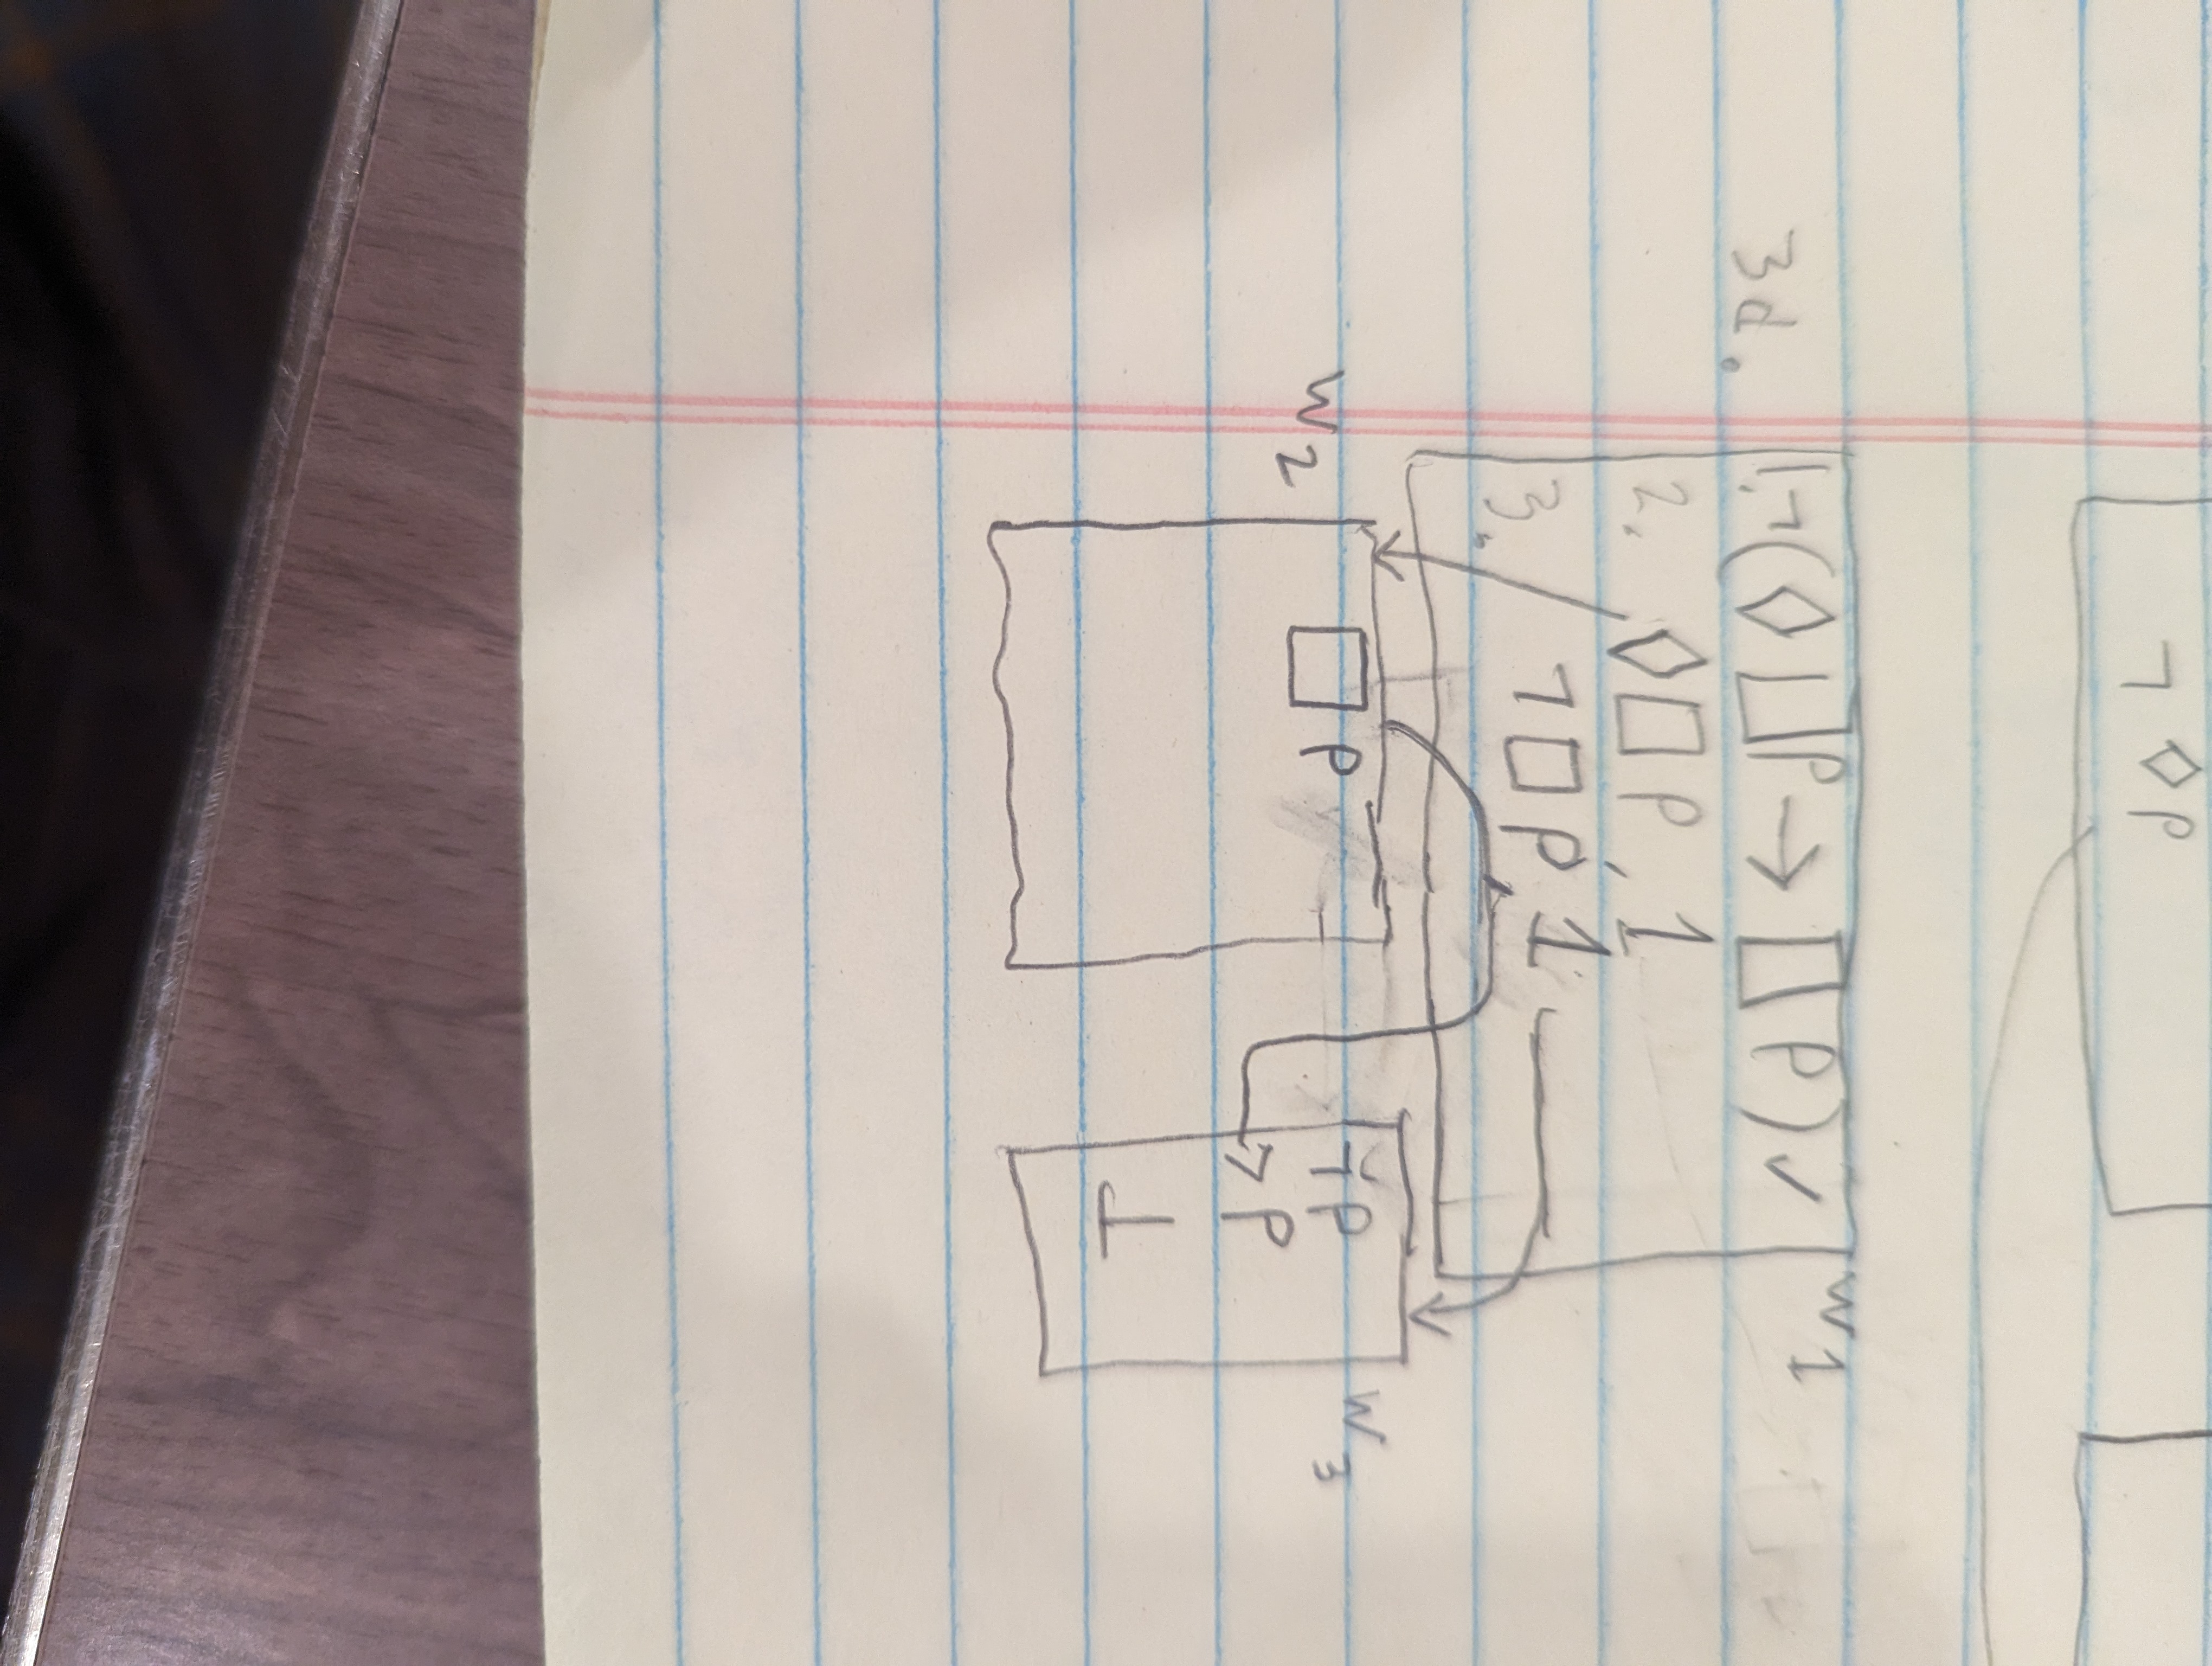
\includegraphics[angle=90,width=\textwidth]{3d}

\section*{Problem 4}

\subsection*{Part A}

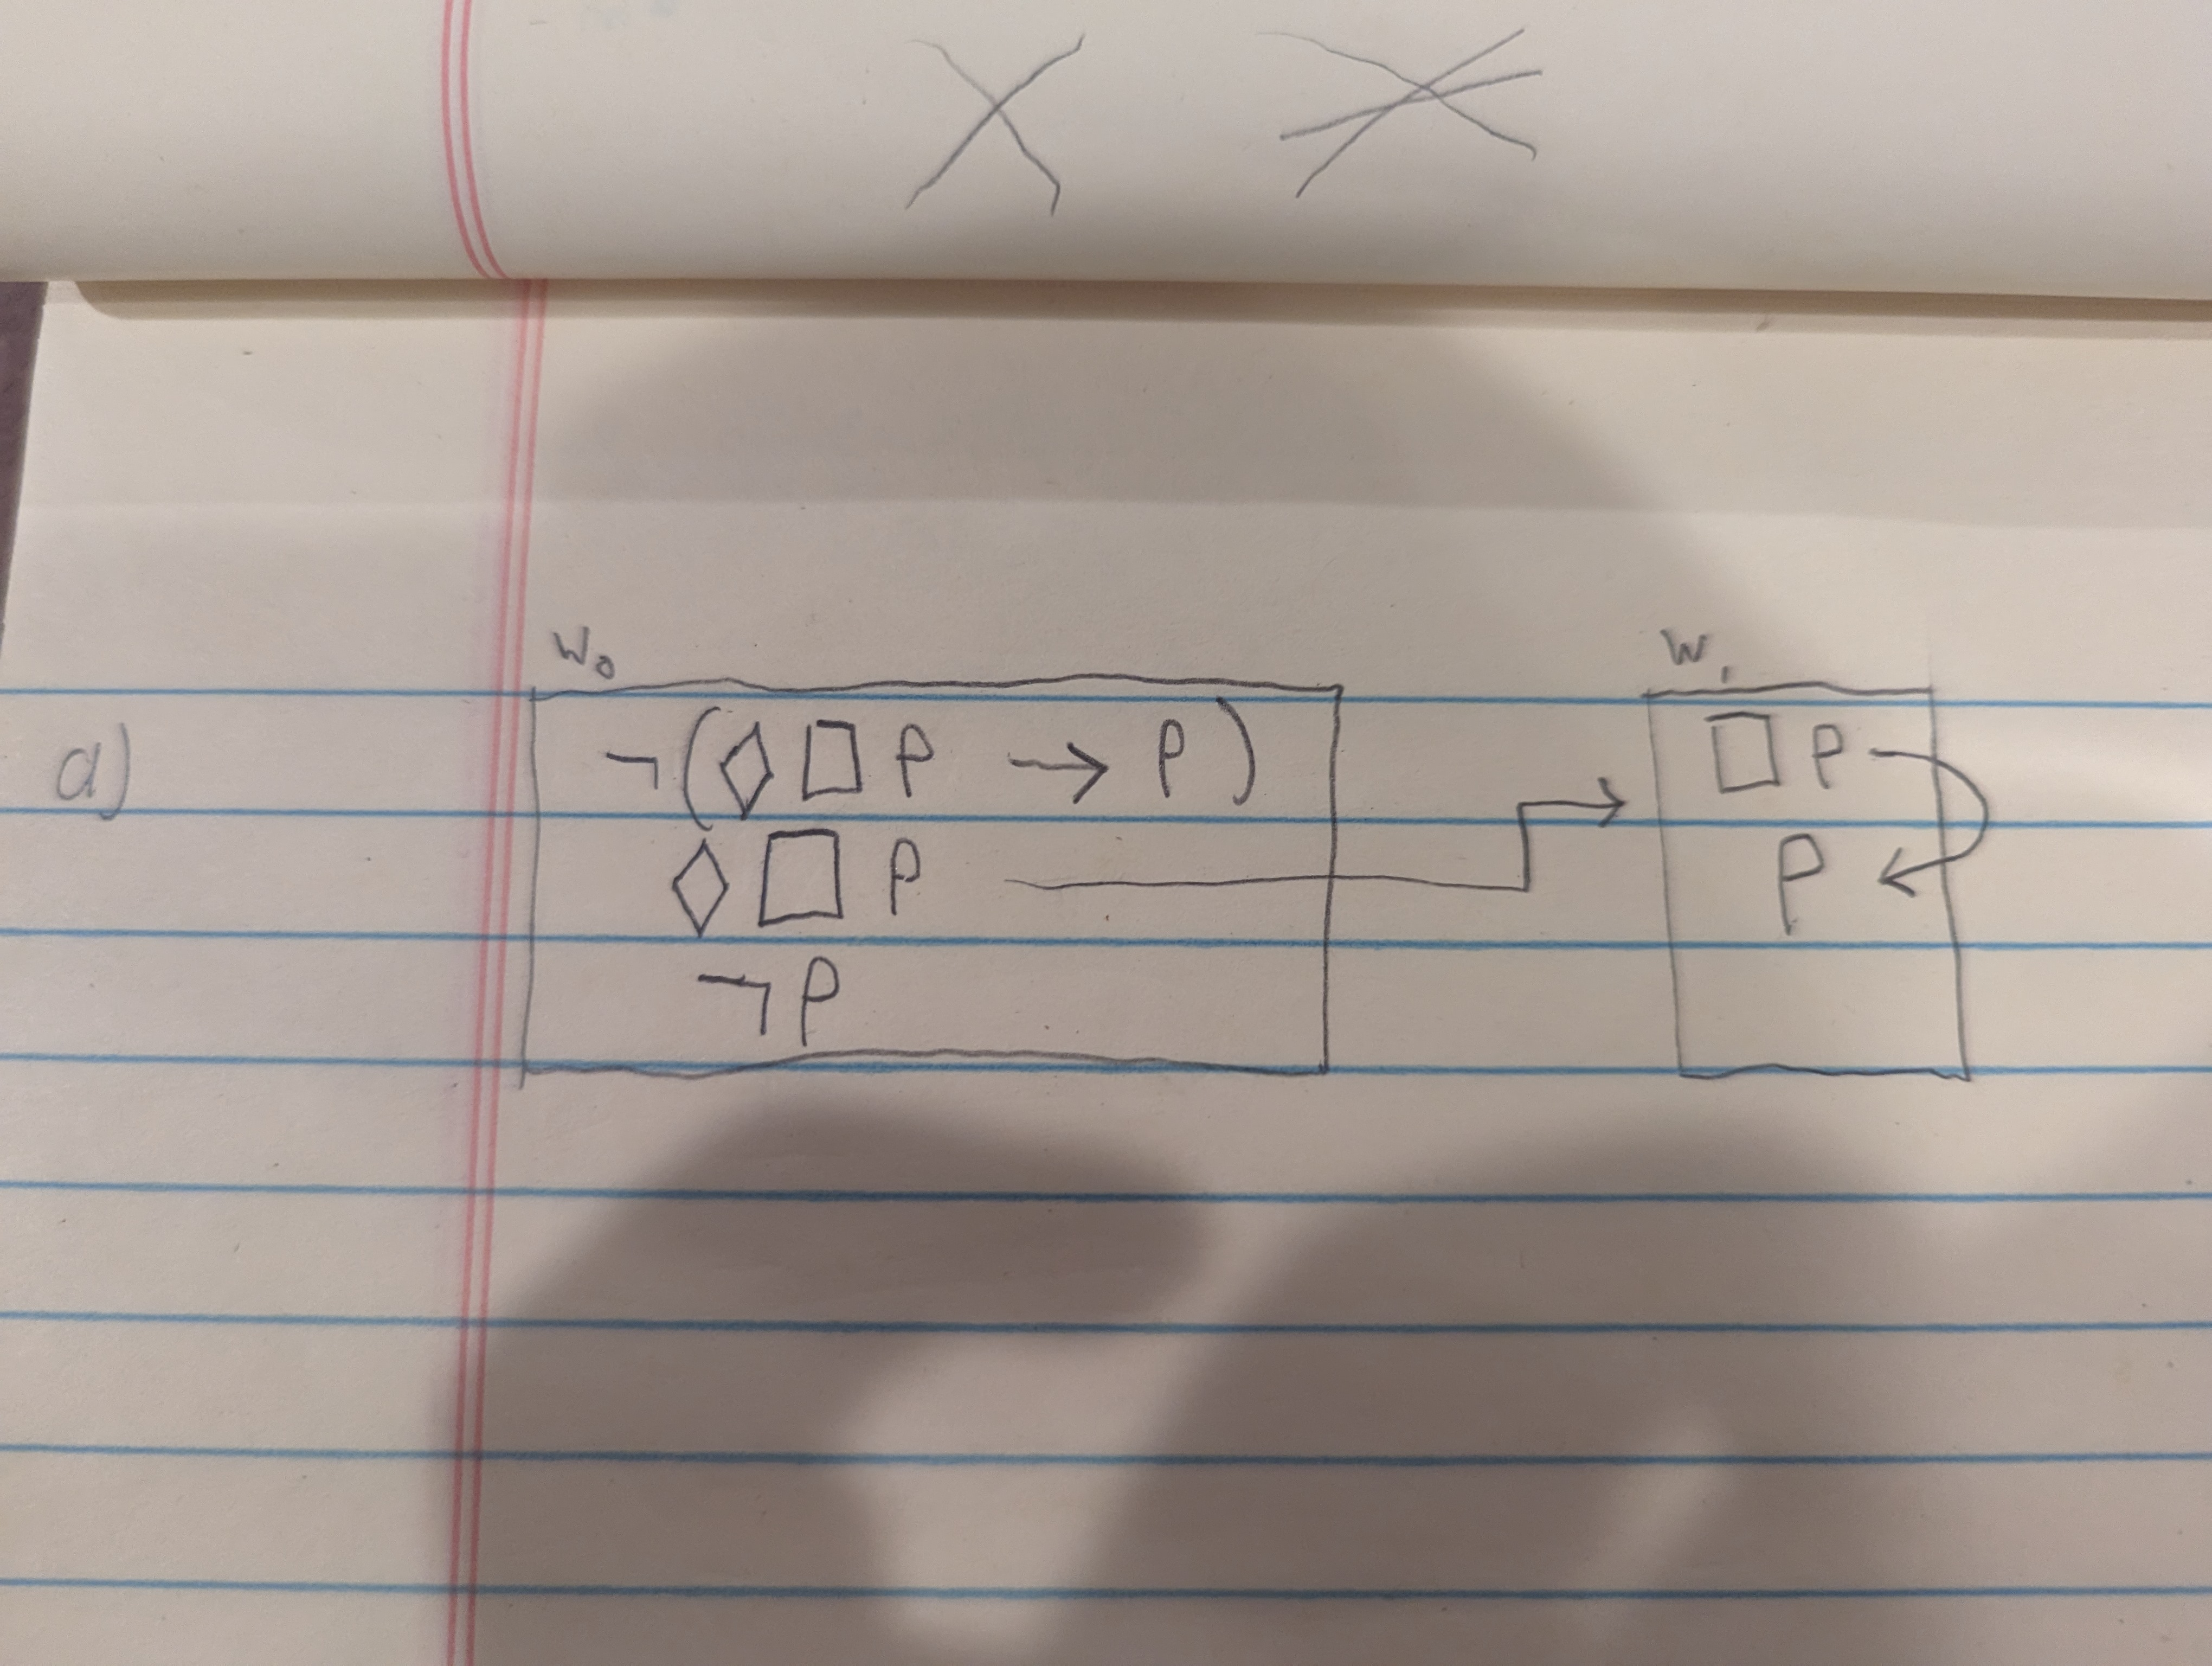
\includegraphics[width=\textwidth]{4a}

A possible interpretation where this statement is false is as followed:
\[ W = \{w_0, w_1\} \]
\[ R = \{(w_0, w_0), (w_1, w_1), (w_0, w_1)\} \]
\[ V(P, w_0) = 0 \]
\[ V(P, w_1) = 1 \]

We can check that $\Diamond \Box P \rightarrow P$ is not a logical truth. 

$\Diamond \Box P$ is true in $w_0$ because there exists a world accessible from $w_1$ where $\Box P$ is true (namely $w_1$)
$P$ is false in $w_0$

So the antecedent is true, and the consequent is false, so the statement is false.

\subsection*{Part B}

\includegraphics[width=\textwidth]{4b}

A possible interpretation where this statement is false is as followed:
\[ W = \{w_0, w_1, w,2\} \]
\[R = \{(w_0, w_1), (w_1, w_0),(w_1, w_2), (w_2, w_1)\} \]
\[ V(P, w_0) = 1 \]
\[ V(P, w_1) = 1 \]
\[ V(P, w_2) = 0 \]

We can check that $\Box P \rightarrow \Box \Box P$ is not true. 

$\Box P$ is true in $w_1$, because $P$ is true in all accessible worlds. 
But $\Box \Box P$ is not true because in $\w_1$ $\Box P$ is not true. 

So the antecedent is true, and the consequent is false, so the statement is false.


\section*{Problem 5}


(a) Every logical truth in K is also a logical truth in $\rho$ 

This is true. 
Something is a logical truth if it is true in all possible worlds. Assume $P$ is a logical truth in K. This means if there were two worlds $W = \{ w_0, w_1 \}$ then $V(P, w_0) = 1$ and $V(P, w_1) = 1$. Adding reflectivity just adds new truths to the worlds, not subtract them. Note that you can end up with contradictions still like if we added $V(\Box \lnot P, w_0) = 1$, then there would be a contradiction only when we add in reflextivity. 

(b) Every sentence that is not a logical truth in S5 is also not a logical truth in s.

This is true. S5 is more powerful than $\sigma$. Removing the ability to access more worlds, just decreases the number of truths, not increases it. So if something is not a true in S5, there is no way that decreasing the amount of worlds that are accessible makes it true. 



\end{document}
